\chapter{Numerical Evaluation: Accuracy and Efficiency}
\label{Chapter4}
\lhead{Chapter 4. \emph{Numerical Evaluation: Accuracy and Efficiency}}

In this chapter, we present a comprehensive analysis of the performance of our newly proposed method with particular focus on its accuracy and efficiency. Through a series of computational experiments, we analyze how different parameters influence the quality of results and CPU-time performance. Specifically, we focus on convergence and the scaling behaviour of our method. All simulations were conducted on ionic systems of sodium (Na\textsuperscript{+}) and chloride (Cl\textsuperscript{-}) ions randomly distributed in a cubic box having a length of 25 \AA. These systems were modelled using the molecular dynamics package LAMMPS~\cite{LAMMPS}. The Ewald splitting parameter $\alpha$ was set to $5.42/L$ as recommended in several previous literature~\cite{frenkel2002understanding}.

The experiments were performed on a machine with a 12-core Intel\textsuperscript{\textregistered} Core\texttrademark{} i5-12500 (12\textsuperscript{th} Gen) processor and 16 GB of RAM. The operating system was OpenSUSE 15.5, and the software used included \texttt{gcc} 7.5.0, FFTW 3.9.9, and GSL 2.6.
\section{Convergence and Accuracy of Reciprocal-Space Contributions with Varying $\gamma$}
In this section, we investigate how the reciprocal-space energy converges as the constant $\gamma$ is varied. A model system of 10000 ions was set up in a box with sides of length 25 \AA. As a benchmark, reference energies were computed using mathematically ``exact'' but computationally inefficient two-dimensional Ewald (2D-EW) method~\cite{kawata2001rapid}.
\subsection{The Role of $\gamma$}
The parameter $\gamma$ plays a central role in controlling the sharpness of the top-hat function that is introduced in the reciprocal sum of 3D Ewald summation method. The introduction of top-hat function filters the interactions arising from interaction of images in the z-direction.  In the new formulation, the long-range part of the Ewald summation is mathematically expressed as
\begin{flalign}
    (4\pi\epsilon_o)U^{LR}& =\frac{\sqrt{\pi}}{L_xL_y}\sum_{\vec{{k}}=-\infty}^{\infty}{}^\prime\left[ \int_{0}^{\alpha}\frac{dt}{t^2}C_{k_z}(t){exp}\left(\frac{-1}{4t^2}|\vec G|_{xy}^2\right)\right] |\,S(\vec G)\,|^2
\end{flalign}
here $\vec k$ = \{$k_x,k_y,k_z$\} and  the constant $\gamma$ appears in the function $C_{k_z}(t)$ given by
\begin{flalign}
     C_{k_z}(t) &=\frac{1}{L_z}\int_{-\infty}^{\infty}ds\hspace{1mm}exp(-i\frac{2\pi n s}{L_z})exp(-s^2t^2)\\
     &\times \left[\frac{1}{1+ exp(-\gamma(0.5L_z+s))} + \frac{1}{1+ exp(-\gamma(0.5L_z-s))} -1\right]
\end{flalign}

\begin{figure}[htbp]
    \centering
    \includegraphics[scale=0.4]{images/logerror_vs_kz_forreport.jpg}
    \caption{Convergence of relative errors in $U_{LR}$ with $k_z$ for various values of $\gamma$.}
    \label{fig:convergence_gamma}
\end{figure}

As shown in Fig.~(\ref{fig:convergence_gamma}) and discussed in Section~\ref{finding_gamma}, the use of different $\gamma$ values significantly influences the rate of convergence of the reciprocal-space energy. Larger $\gamma$ values lead to relatively faster convergence but introduce oscillatory behaviour in the energy estimates with low accuracy, contrary to smaller values, which have high accuracy and fewer oscillations. To achieve convergence in energies, one needs to reach a threshold $k_z$. Consequently, this brings a major drawback: for every additional iteration of $k_z$ in the main energy summation, the structure factor $S(\vec G)$~Eq.(\ref{eq:structurefactor}) is recomputed, which scales as $O(N)$, adding to the computational overhead for high precision simulations. 

To eliminate this cost, we transition to the use of the Particle Mesh adaptation of our new method, as formulated in Eq.~(\ref{eq:newreci2DSPME}). In this formulation, the most computationally expensive step becomes the charge interpolation on grids, which is executed only once and outside the main energy summation loop. As a result, the main energy summation loop is no longer the computational bottleneck, enabling significantly faster calculations without sacrificing accuracy.

\section{Implementation with Particle Mesh Ewald}
The Particle Mesh Ewald formulation introduces several additional parameters that directly impacts both computational efficiency and numerical accuracy. They are the resolution of the mesh grid used for the Fast Fourier Transform (FFT) and the order of the B-spline interpolation for charge assignment. In this section, we systematically investigate how variations in these parameters affect the performance of our method, particularly in conjunction with different values of parameter $\gamma$.

In our modified implementation, we performed extensive tests across a variety of $\gamma$ values, grid sizes, and B-spline interpolation orders. For each configuration, we measured the accuracy of the computed electrostatic energy and recorded the CPU execution time. These combinations are presented in the Tables~\ref{tab:tablespme_gamma0p2}, \ref{tab:tablespme_gamma0p5}, \ref{tab:tablespme_gamma1}, \ref{tab:tablespme_gamma2p5}, and \ref{tab:tablespme_gamma10}

\begin{table}[H]
\centering
\begin{tabular}{|l|c|l|}
\hline
\textbf{Color Code}      & \textbf{Accuracy} & \textbf{Rel. Err. Range}                                      \\ \hline
\cellcolor[HTML]{F0F7DA} & Low               & More than $10^{-4}$                      \\ \hline
\cellcolor[HTML]{C9DF8A} & Medium            & Between $10^{-6}$ and $10^{-4}$ \\ \hline
\cellcolor[HTML]{77AB59} & High              & Less than $10^{-6}$                      \\ \hline
\end{tabular}
\caption{Color-coded accuracy classification for the SPME method based on error range}
\label{tab:accuracy-refer}
\end{table}
% high  77AB59
% mid C9DF8A
% low F0F7DA
\begin{table}[]
\centering
\caption{Particle Mesh Method: performance and accuracy for $\gamma = 0.2$.}
\label{tab:tablespme_gamma0p2}
\resizebox{\textwidth}{!}{%
\begin{tabular}{cccccc}
\hline
\multicolumn{1}{|c|}{{Order$_{xy}$}} &
  \multicolumn{1}{c|}{{Order$_z$}} &
  \multicolumn{1}{c|}{{Grid$_{xy}$}} &
  \multicolumn{1}{c|}{{Grid$_z$}} &
  \multicolumn{1}{c|}{{\begin{tabular}[c]{@{}c@{}}CPU-Time\\ (sec)\end{tabular}}} &
  \multicolumn{1}{c|}{{\begin{tabular}[c]{@{}c@{}}Rel. Err.\\ Energy\end{tabular}}} \\ \hline
\rowcolor[HTML]{F0F7DA} 
4  & 4  & 16 & 512 & 0.0748 & 4.4E-04 \\
\rowcolor[HTML]{C9DF8A} 
4  & 4  & 32 & 512 & 0.0805 & 4.2E-05 \\
\rowcolor[HTML]{C9DF8A} 
4  & 4  & 64 & 512 & 0.1076 & 1.8E-05 \\
\rowcolor[HTML]{F0F7DA} 
4  & 6  & 16 & 512 & 0.0751 & 4.2E-04 \\
\rowcolor[HTML]{C9DF8A} 
4  & 6  & 32 & 512 & 0.0807 & 2.6E-05 \\
\rowcolor[HTML]{C9DF8A} 
4  & 6  & 64 & 512 & 0.1090 & 1.8E-06 \\
\rowcolor[HTML]{F0F7DA} 
4  & 8  & 16 & 512 & 0.0810 & 4.2E-04 \\
\rowcolor[HTML]{C9DF8A} 
4  & 8  & 32 & 512 & 0.0868 & 2.6E-05 \\
\rowcolor[HTML]{C9DF8A} 
4  & 8  & 64 & 512 & 0.1162 & 1.7E-06 \\
\rowcolor[HTML]{F0F7DA} 
4  & 10 & 16 & 512 & 0.1060 & 4.2E-04 \\
\rowcolor[HTML]{C9DF8A} 
4  & 10 & 32 & 512 & 0.1118 & 2.6E-05 \\
\rowcolor[HTML]{C9DF8A} 
4  & 10 & 64 & 512 & 0.1391 & 1.7E-06 \\
\rowcolor[HTML]{C9DF8A} 
6  & 6  & 16 & 512 & 0.1260 & 1.3E-05 \\
\rowcolor[HTML]{77AB59} 
6  & 6  & 32 & 512 & 0.1328 & 4.0E-07 \\
\rowcolor[HTML]{77AB59} 
6  & 6  & 64 & 512 & 0.1709 & 2.7E-07 \\
\rowcolor[HTML]{C9DF8A} 
6  & 8  & 16 & 512 & 0.1322 & 1.3E-05 \\
\rowcolor[HTML]{77AB59} 
6  & 8  & 32 & 512 & 0.1401 & 3.0E-07 \\
\rowcolor[HTML]{77AB59} 
6  & 8  & 64 & 512 & 0.1788 & 1.7E-07 \\
\rowcolor[HTML]{C9DF8A} 
6  & 10 & 16 & 512 & 0.1580 & 1.3E-05 \\
\rowcolor[HTML]{77AB59} 
6  & 10 & 32 & 512 & 0.1637 & 3.0E-07 \\
\rowcolor[HTML]{77AB59} 
6  & 10 & 64 & 512 & 0.2027 & 1.7E-07 \\
\rowcolor[HTML]{77AB59} 
8  & 8  & 32 & 512 & 0.2182 & 1.7E-07 \\
\rowcolor[HTML]{77AB59} 
8  & 8  & 64 & 512 & 0.2701 & 1.7E-07 \\
\rowcolor[HTML]{77AB59} 
8  & 10 & 32 & 512 & 0.2444 & 1.7E-07 \\
\rowcolor[HTML]{77AB59} 
8  & 10 & 64 & 512 & 0.2999 & 1.6E-07 \\
\rowcolor[HTML]{77AB59} 
10 & 10 & 64 & 512 & 0.4521 & 1.6E-07
\end{tabular}%
}
\end{table}
% high  77AB59
% mid C9DF8A
% low F0F7DA
\begin{table}[]
\centering
\caption{Particle Mesh Method: performance and accuracy for $\gamma = 0.5$.}
\label{tab:tablespme_gamma0p5}
\resizebox{\textwidth}{!}{%
\begin{tabular}{cccccc}
\hline
\multicolumn{1}{|c|}{{Order$_{xy}$}} &
  \multicolumn{1}{c|}{{Order$_z$}} &
  \multicolumn{1}{c|}{{Grid$_{xy}$}} &
  \multicolumn{1}{c|}{{Grid$_z$}} &
  \multicolumn{1}{c|}{{\begin{tabular}[c]{@{}c@{}}CPU-Time\\ (sec)\end{tabular}}} &
  \multicolumn{1}{c|}{{\begin{tabular}[c]{@{}c@{}}Rel. Err.\\ Energy\end{tabular}}} \\ \hline
\rowcolor[HTML]{F0F7DA} 
4  & 4  & 16  & 256 & 0.0426 & 4.4E-04 \\
\rowcolor[HTML]{C9DF8A} 
4  & 4  & 32  & 256 & 0.0465 & 4.0E-05 \\
\rowcolor[HTML]{C9DF8A} 
4  & 4  & 64  & 256 & 0.0599 & 1.5E-05 \\
\rowcolor[HTML]{F0F7DA} 
4  & 6  & 16  & 256 & 0.0436 & 4.2E-04 \\
\rowcolor[HTML]{C9DF8A} 
4  & 6  & 32  & 256 & 0.0479 & 2.6E-05 \\
\rowcolor[HTML]{C9DF8A} 
4  & 6  & 64  & 256 & 0.0611 & 1.7E-06 \\
\rowcolor[HTML]{F0F7DA} 
4  & 8  & 16  & 256 & 0.0497 & 4.2E-04 \\
\rowcolor[HTML]{C9DF8A} 
4  & 8  & 32  & 256 & 0.0539 & 2.6E-05 \\
\rowcolor[HTML]{C9DF8A} 
4  & 8  & 64  & 256 & 0.0667 & 1.6E-06 \\
\rowcolor[HTML]{F0F7DA} 
4  & 10 & 16  & 256 & 0.0742 & 4.2E-04 \\
\rowcolor[HTML]{C9DF8A} 
4  & 10 & 32  & 256 & 0.0783 & 2.6E-05 \\
\rowcolor[HTML]{C9DF8A} 
4  & 10 & 64  & 256 & 0.0914 & 1.6E-06 \\
\rowcolor[HTML]{C9DF8A} 
6  & 6  & 16  & 256 & 0.0720 & 1.3E-05 \\
\rowcolor[HTML]{77AB59} 
6  & 6  & 32  & 256 & 0.0767 & 2.9E-07 \\
\rowcolor[HTML]{77AB59} 
6  & 6  & 64  & 256 & 0.0923 & 1.6E-07 \\
\rowcolor[HTML]{C9DF8A} 
6  & 8  & 16  & 256 & 0.0788 & 1.3E-05 \\
\rowcolor[HTML]{77AB59} 
6  & 8  & 32  & 256 & 0.0833 & 2.2E-07 \\
\rowcolor[HTML]{77AB59} 
6  & 8  & 64  & 256 & 0.0968 & 8.7E-08 \\
\rowcolor[HTML]{C9DF8A} 
6  & 10 & 16  & 256 & 0.1038 & 1.3E-05 \\
\rowcolor[HTML]{77AB59} 
6  & 10 & 32  & 256 & 0.1074 & 2.2E-07 \\
\rowcolor[HTML]{77AB59} 
6  & 10 & 64  & 256 & 0.1234 & 8.6E-08 \\
\rowcolor[HTML]{77AB59} 
8  & 8  & 32  & 256 & 0.1319 & 8.6E-08 \\
\rowcolor[HTML]{77AB59} 
8  & 8  & 64  & 256 & 0.1489 & 8.5E-08 \\
\rowcolor[HTML]{77AB59} 
8  & 10 & 32  & 256 & 0.1555 & 8.6E-08 \\
\rowcolor[HTML]{77AB59} 
8  & 10 & 64  & 256 & 0.1782 & 8.4E-08 \\
\rowcolor[HTML]{77AB59} 
10 & 10 & 128 & 256 & 0.3718 & 8.4E-08
\end{tabular}%
}
\end{table}
% high  77AB59
% mid C9DF8A
% low F0F7DA
\begin{table}[]
\centering
\caption{Particle Mesh Method: performance and accuracy for $\gamma = 1.0$.}
\label{tab:tablespme_gamma1}
\resizebox{\textwidth}{!}{%
\begin{tabular}{cccccc}
\hline
\multicolumn{1}{|c|}{{Order$_{xy}$}} &
  \multicolumn{1}{c|}{{Order$_z$}} &
  \multicolumn{1}{c|}{{Grid$_{xy}$}} &
  \multicolumn{1}{c|}{{Grid$_z$}} &
  \multicolumn{1}{c|}{{\begin{tabular}[c]{@{}c@{}}CPU-Time\\ (sec)\end{tabular}}} &
  \multicolumn{1}{c|}{{\begin{tabular}[c]{@{}c@{}}Rel. Err.\\ Energy\end{tabular}}} \\ \hline
\rowcolor[HTML]{F0F7DA} 
4  & 4  & 16 & 128 & 0.0262 & 4.6E-04 \\
\rowcolor[HTML]{C9DF8A} 
4  & 4  & 32 & 128 & 0.0294 & 6.5E-05 \\
\rowcolor[HTML]{C9DF8A} 
4  & 4  & 64 & 128 & 0.0373 & 4.1E-05 \\
\rowcolor[HTML]{F0F7DA} 
4  & 6  & 16 & 128 & 0.0276 & 4.2E-04 \\
\rowcolor[HTML]{C9DF8A} 
4  & 6  & 32 & 128 & 0.0308 & 2.6E-05 \\
\rowcolor[HTML]{C9DF8A} 
4  & 6  & 64 & 128 & 0.0387 & 2.0E-06 \\
\rowcolor[HTML]{F0F7DA} 
4  & 8  & 16 & 128 & 0.0337 & 4.2E-04 \\
\rowcolor[HTML]{C9DF8A} 
4  & 8  & 32 & 128 & 0.0369 & 2.6E-05 \\
\rowcolor[HTML]{C9DF8A} 
4  & 8  & 64 & 128 & 0.0447 & 1.6E-06 \\
\rowcolor[HTML]{F0F7DA} 
4  & 10 & 16 & 128 & 0.0586 & 4.2E-04 \\
\rowcolor[HTML]{C9DF8A} 
4  & 10 & 32 & 128 & 0.0614 & 2.6E-05 \\
\rowcolor[HTML]{C9DF8A} 
4  & 10 & 64 & 128 & 0.0693 & 1.6E-06 \\
\rowcolor[HTML]{C9DF8A} 
6  & 6  & 16 & 128 & 0.0452 & 1.3E-05 \\
\rowcolor[HTML]{77AB59} 
6  & 6  & 32 & 128 & 0.0481 & 6.1E-07 \\
\rowcolor[HTML]{77AB59} 
6  & 6  & 64 & 128 & 0.0564 & 4.8E-07 \\
\rowcolor[HTML]{C9DF8A} 
6  & 8  & 16 & 128 & 0.0517 & 1.3E-05 \\
\rowcolor[HTML]{77AB59} 
6  & 8  & 32 & 128 & 0.0546 & 2.3E-07 \\
\rowcolor[HTML]{77AB59} 
6  & 8  & 64 & 128 & 0.0626 & 9.9E-08 \\
\rowcolor[HTML]{C9DF8A} 
6  & 10 & 16 & 128 & 0.0761 & 1.3E-05 \\
\rowcolor[HTML]{77AB59} 
6  & 10 & 32 & 128 & 0.0802 & 2.3E-07 \\
\rowcolor[HTML]{77AB59} 
6  & 10 & 64 & 128 & 0.0876 & 9.2E-08 \\
\rowcolor[HTML]{77AB59} 
8  & 8  & 32 & 128 & 0.0859 & 9.8E-08 \\
\rowcolor[HTML]{77AB59} 
8  & 8  & 64 & 128 & 0.0942 & 9.7E-08 \\
\rowcolor[HTML]{77AB59} 
8  & 10 & 32 & 128 & 0.1105 & 9.2E-08 \\
\rowcolor[HTML]{77AB59} 
8  & 10 & 64 & 128 & 0.1194 & 9.1E-08 \\
\rowcolor[HTML]{77AB59} 
10 & 10 & 64 & 128 & 0.1941 & 9.1E-08
\end{tabular}%
}
\end{table}
% high  77AB59
% mid C9DF8A
% low F0F7DA
\begin{table}[]
\centering
\caption{Particle Mesh Method: performance and accuracy for $\gamma = 2.5$.}
\label{tab:tablespme_gamma2p5}
\resizebox{\textwidth}{!}{%
\begin{tabular}{cccccc}
\hline
\multicolumn{1}{|c|}{{Order$_{xy}$}} &
  \multicolumn{1}{c|}{{Order$_z$}} &
  \multicolumn{1}{c|}{{Grid$_{xy}$}} &
  \multicolumn{1}{c|}{{Grid$_z$}} &
  \multicolumn{1}{c|}{{\begin{tabular}[c]{@{}c@{}}CPU-Time\\ (sec)\end{tabular}}} &
  \multicolumn{1}{c|}{{\begin{tabular}[c]{@{}c@{}}Rel. Err.\\ Energy\end{tabular}}} \\ \hline
\rowcolor[HTML]{F0F7DA} 
4  & 4  & 16 & 128 & 0.0276  & 4.3E-04 \\
\rowcolor[HTML]{C9DF8A} 
4  & 4  & 32 & 128 & 0.0313  & 3.3E-05 \\
\rowcolor[HTML]{C9DF8A} 
4  & 4  & 64 & 128 & 0.0396  & 9.1E-06 \\
\rowcolor[HTML]{F0F7DA} 
4  & 8  & 16 & 128 & 0.0357  & 4.3E-04 \\
\rowcolor[HTML]{C9DF8A} 
4  & 8  & 32 & 128 & 0.0388  & 2.7E-05 \\
\rowcolor[HTML]{C9DF8A} 
4  & 8  & 64 & 128 & 0.0478  & 3.1E-06 \\
\rowcolor[HTML]{F0F7DA} 
4  & 10 & 16 & 128 & 0.0613  & 4.3E-04 \\
\rowcolor[HTML]{C9DF8A} 
4  & 10 & 32 & 128 & 0.0653  & 2.7E-05 \\
\rowcolor[HTML]{C9DF8A} 
4  & 10 & 64 & 128 & 0.0722  & 3.1E-06 \\
\rowcolor[HTML]{C9DF8A} 
6  & 8  & 16 & 128 & 0.0534  & 1.5E-05 \\
\rowcolor[HTML]{C9DF8A} 
6  & 8  & 32 & 128 & 0.0567  & 1.7E-06 \\
\rowcolor[HTML]{C9DF8A} 
6  & 8  & 64 & 128 & 0.0652  & 1.5E-06 \\
\rowcolor[HTML]{C9DF8A} 
6  & 10 & 16 & 128 & 0.0798  & 1.5E-05 \\
\rowcolor[HTML]{C9DF8A} 
6  & 10 & 32 & 128 & 0.0824  & 1.7E-06 \\
\rowcolor[HTML]{C9DF8A} 
6  & 10 & 64 & 128 & 0.0909  & 1.5E-06 \\
\rowcolor[HTML]{C9DF8A} 
8  & 8  & 32 & 128 & 0.0936  & 1.5E-06 \\
\rowcolor[HTML]{C9DF8A} 
8  & 8  & 64 & 128 & 0.1037  & 1.5E-06 \\
\rowcolor[HTML]{C9DF8A} 
8  & 10 & 64 & 128 & 0.12805 & 1.5E-06 \\
\rowcolor[HTML]{C9DF8A} 
10 & 10 & 64 & 128 & 0.20766 & 1.5E-06
\end{tabular}%
}
\end{table}
% high  77AB59
% mid C9DF8A
% low F0F7DA
\begin{table}[]
\centering
\caption{Particle Mesh Method: performance and accuracy for $\gamma = 10$.}
\label{tab:tablespme_gamma10}
\resizebox{\textwidth}{!}{%
\begin{tabular}{cccccc}
\hline
\multicolumn{1}{|c|}{{Order$_{xy}$}} &
  \multicolumn{1}{c|}{{Order$_z$}} &
  \multicolumn{1}{c|}{{Grid$_{xy}$}} &
  \multicolumn{1}{c|}{{Grid$_z$}} &
  \multicolumn{1}{c|}{{\begin{tabular}[c]{@{}c@{}}CPU-Time\\ (sec)\end{tabular}}} &
  \multicolumn{1}{c|}{{\begin{tabular}[c]{@{}c@{}}Rel. Err.\\ Energy\end{tabular}}} \\ \hline
\rowcolor[HTML]{F0F7DA} 
4  & 4  & 16 & 128 & 0.0276 & 4.8E-04 \\
\rowcolor[HTML]{C9DF8A} 
4  & 4  & 32 & 128 & 0.0309 & 8.1E-05 \\
\rowcolor[HTML]{C9DF8A} 
4  & 4  & 64 & 128 & 0.0389 & 5.6E-05 \\
\rowcolor[HTML]{F0F7DA} 
4  & 8  & 16 & 128 & 0.0358 & 4.8E-04 \\
\rowcolor[HTML]{C9DF8A} 
4  & 8  & 64 & 128 & 0.0476 & 5.5E-05 \\
\rowcolor[HTML]{F0F7DA} 
4  & 10 & 16 & 128 & 0.0618 & 4.8E-04 \\
\rowcolor[HTML]{C9DF8A} 
4  & 10 & 64 & 128 & 0.0734 & 5.4E-05 \\
\rowcolor[HTML]{C9DF8A} 
6  & 8  & 64 & 128 & 0.0675 & 5.3E-05 \\
\rowcolor[HTML]{C9DF8A} 
6  & 10 & 64 & 128 & 0.0939 & 5.3E-05 \\
\rowcolor[HTML]{C9DF8A} 
8  & 8  & 64 & 128 & 0.1025 & 5.3E-05 \\
\rowcolor[HTML]{C9DF8A} 
8  & 10 & 64 & 128 & 0.1284 & 5.3E-05 \\
\rowcolor[HTML]{C9DF8A} 
10 & 10 & 64 & 128 & 0.2109 & 5.3E-05
\end{tabular}%
}
\end{table}

Several general trends emerged from the analysis. Lower values of $\gamma$ were found to require finer grids in the $ z$-direction in order to achieve a comparable level of accuracy, which in turn increases the computational cost. Increasing the B-spline interpolation order generally improves the accuracy of the energy calculations; however, that effect diminishes beyond a certain order while the computational overhead continues to increase. While multiple configurations may yield acceptable results, the combination of $\gamma = 1$ or $0.5$, a grid size of $64 \times 64 \times 128$, and a B-spline interpolation order of 8 was found to offer the most favourable balance between numerical accuracy and computational efficiency among the cases evaluated.

\section{Scaling Behaviour with System Size}
To evaluate the scalability of our method with respect to system size, we analyzed the computational performance of the PME implementation of our method. The number of ions were varied from 1,000 to 30,000, with particle positions randomly distributed within a fixed simulation box. Throughout all simulations, the PME configuration was kept uniform with a grid size of $64 \times 64 \times 128$, a B-spline interpolation order of 8, and $\gamma = 1$, as identified in the previous section. For comparison, we also included results from previously established methods based on 2D and 3D periodic boundary conditions, with particle mesh adaptation for a similar level of accuracy. The scaling behavior of the total computation time with increasing system size is shown in Fig.~(\ref{fig:scaling_results}). 
\begin{figure}[]
    \centering
    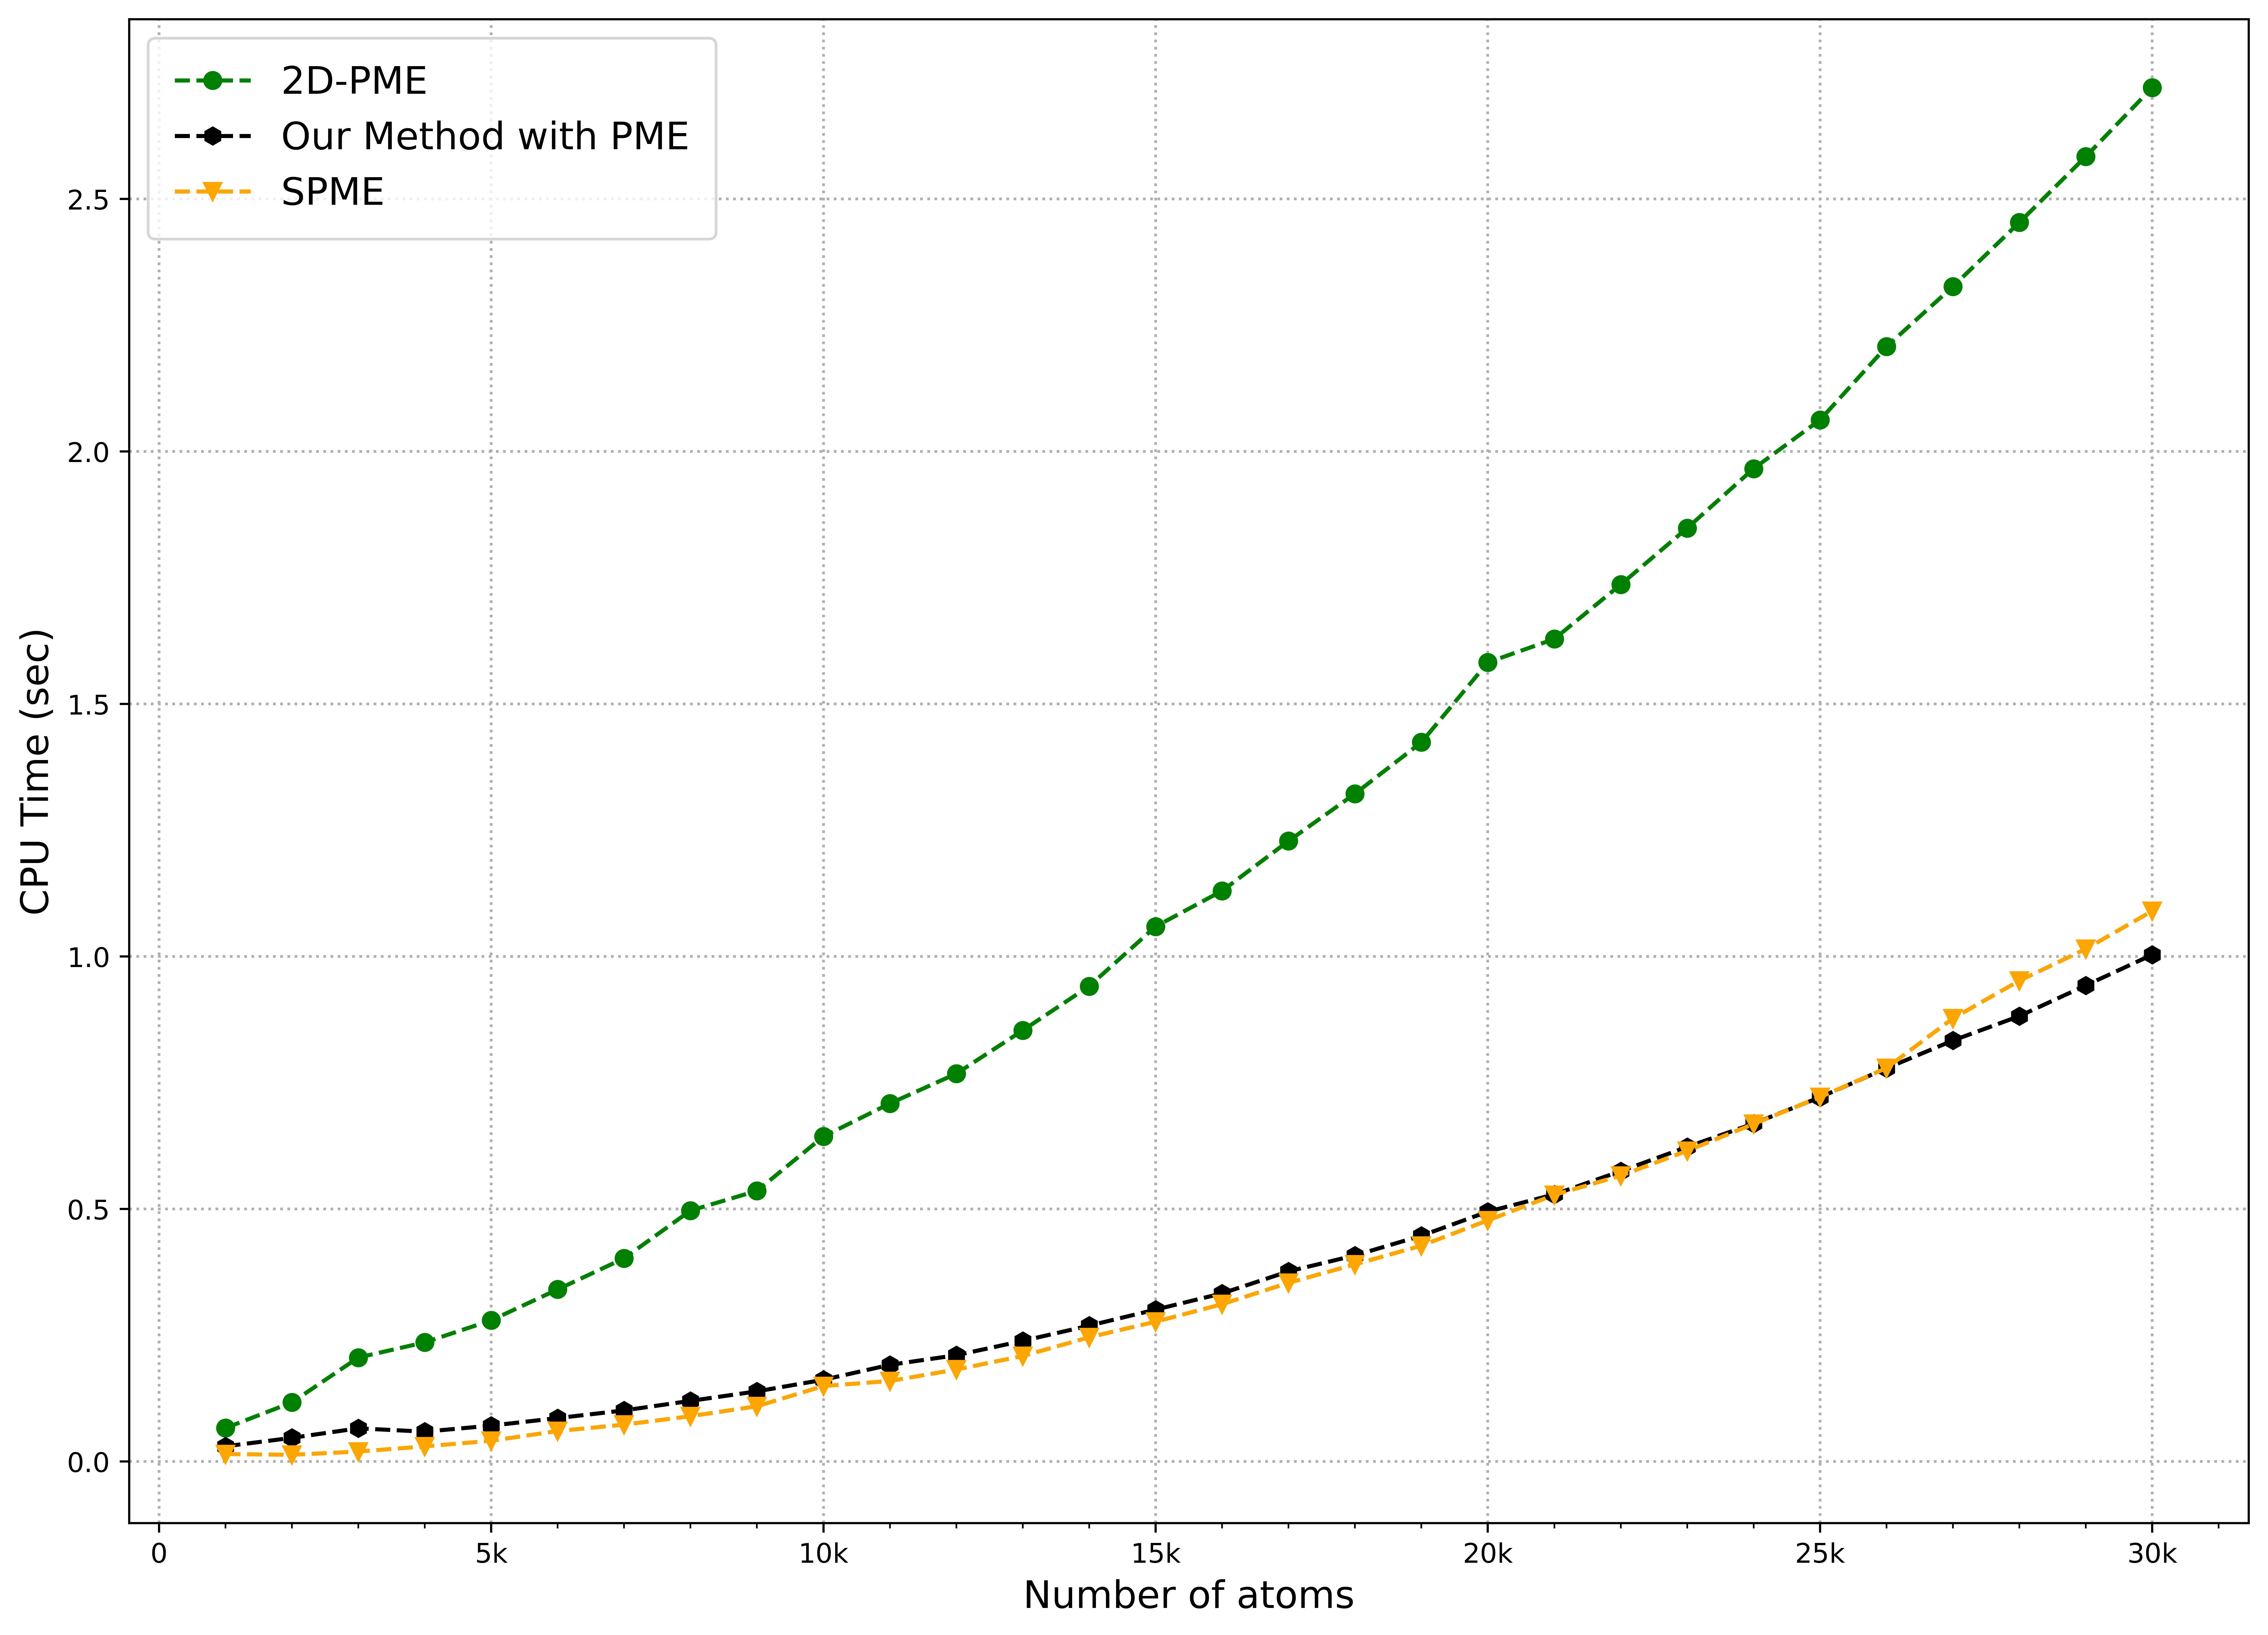
\includegraphics[width=\linewidth]{images/Scaling_behaviour_Result30k.jpg}
    \caption{Scaling behaviour of the computation time for total Ewald energies with increasing system size for the optimized PME implementation. The number of ions was varied from 1,000 to 30,000 while keeping the simulation box size fixed.  Our method demonstrated highly improved performance compared to the conventional \ac{2D-PME} approach and a similar performance to 3D-\ac{SPME}, using the same particle mesh configuration and achieving a comparable level of accuracy.}
    \label{fig:scaling_results}
\end{figure}
Our method shows a substantial improvement in computational efficiency compared to the conventional \ac{2D-PME} method. The scaling of the CPU time is significantly better as shown with the slower growth of the computational time in our method's curve. This enhanced performance can be attributed to the 3D-\ac{SPME} like formulation of our new method, which is evident as both show a similar performance. Since the 3D-SPME method is known for its scalability and accuracy, our implementation matches its performance while providing adaptability to slab-like geometries often encountered in biological and interfacial simulations. 